\chapter{圆}
在工农业生产和日常生活中,圆的应用相当广泛。过去
我们初步掌握了一些圆的知识,这一章我们将在复习这些知
识的基础上,把圆和直线形结合起来,进一步学习有关圆的
一些性质。

\section{圆的基本性质}
\subsection{圆的概念}
在一个平面上和某一定点的距离等于定长的点的集合叫
做\textbf{圆周},简称为\textbf{圆};其中定点叫做圆的\textbf{圆心},连结圆心与圆
上任一点的线段叫做\textbf{半径}.通常以点$O$为圆心的圆记作$\odot O$; 
以点$O$为圆心,半径长是$r$的圆记作$\odot(O,r)$。


显然,\textbf{同圆的半径都相等}(图4.1)。而当一个圆的圆
心确定了,半径$r$的大小也确定了,这个圆的位置与大小也
就完全确定了。

圆上任意两点间的部分叫做\textbf{弧};连结圆上任意两点间的
线段叫做这个圆的弦;通过圆心的弦叫做圆的\textbf{直径}(图4.2)。
显然,\textbf{一个圆的直径等于它的半径的二倍}。
\begin{figure}[htp]\centering
    \begin{minipage}[t]{0.48\textwidth}
    \centering
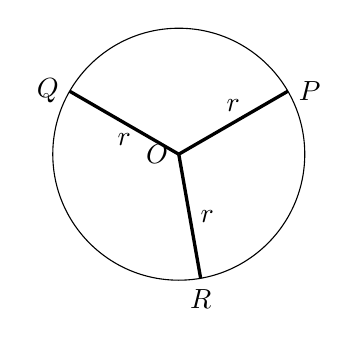
\begin{tikzpicture}[>=latex, scale=.8]
    \draw (0,0) circle (2);
\draw[very thick](0,0)node[left]{$O$}--node[above]{$r$}(30:2)node[right]{$P$};
\draw[very thick](0,0)--node[below]{$r$}(150:2)node[left]{$Q$};
\draw[very thick](0,0)--node[right]{$r$}(-80:2)node[below]{$R$};
    \end{tikzpicture}
    \caption{}
    \end{minipage}
    \begin{minipage}[t]{0.48\textwidth}
    \centering
    \begin{tikzpicture}[>=latex, scale=.8]
        \draw  (0,0) circle (2);
\draw[very thick] (60:2)--node[below]{弦}(135:2);
\draw[very thick] (-10:2)--node[below]{直径}(170:2);
\draw (-135:2) [fill=black]circle(1.5pt)node[left]{$E$};
\draw (-45:2) [fill=black]circle(1.5pt)node[right]{$F$};
\draw[very thick]  (-135:2) arc (-135:-45:2);
\node at (0,-2) [below=2pt]{弧};


    \end{tikzpicture}
    \caption{}
    \end{minipage}
    \end{figure}

从圆的定义,不难直接推知:
\begin{itemize}
    \item 两个圆能够重合的充要条件是两个圆的半径相等。
    \item 半径相等的圆叫做\textbf{等圆},\textbf{等圆的半径相等直径相等}。
\end{itemize}

从圆的定义,我们还可以看出,一个圆把它所在的平面
分为三部分(图4.3):
\begin{enumerate}
    \item 圆本身,即与圆心的距离等于半径的点所构成的集
合。其中任何一点都叫做圆上的点。
\item 圆的内部,与圆心的距离小于半径的点所构成的集
合。圆的内部又简称\textbf{圆内};其中任何一点都叫做圆内的点。
\item 圆的外部:与圆心的距离大于半径的点所构成的集
合;圆的外部又简称\textbf{圆外},其中任何一点都叫做圆外的点。
\end{enumerate}

\begin{figure}[htp]\centering
    \begin{minipage}[t]{0.48\textwidth}
    \centering
\begin{tikzpicture}[>=latex, scale=.8]
    \draw[pattern=north west lines] (0,0) circle (2);
    \draw[thick] (0,0)--node[left=3.5pt, fill=white]{$r$}(60:2);
    \end{tikzpicture}
    \caption{}
    \end{minipage}
    \begin{minipage}[t]{0.48\textwidth}
    \centering
    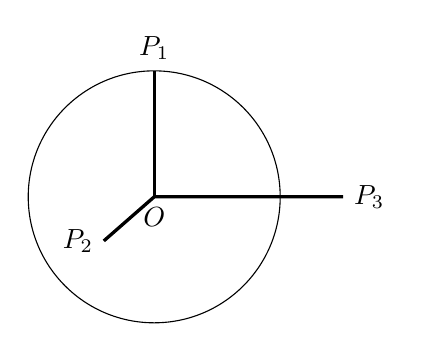
\begin{tikzpicture}[>=latex, scale=.8]
        \draw  (0,0) circle (2);
\draw[very thick](-.8,-.7)node[left]{$P_2$}--(0,0)node[below]{$O$}--(3,0)node[right]{$P_3$};
\draw[very thick](0,0)--(0,2)node[above]{$P_1$};

    \end{tikzpicture}
    \caption{}
    \end{minipage}
    \end{figure}

通常我们说的圆面,指的是由圆所围成的平面部分,也
就是与圆心的距离小于或等于半径的点所构成的集合。如图
4.3中阴影部分。

由上述定义可知,$\odot(O,r)$与平面上任一点P的位置关
系,有下述的性质(图4.4)。
\begin{enumerate}
    \item 点$P$在$\odot(O,r)$上的充要条件是$\overline{OP}=r$;
    \item 点$P$在$\odot(O,r)$内的充要条件是$\overline{OP}<r$;
    \item 点$P$在$\odot(O,r)$外的充要条件是$\overline{OP}>r$。
\end{enumerate}

\begin{ex}
\begin{enumerate}
    \item 根据下述条件画圆
\begin{enumerate}
\item 已知定点$O$, 以$O$为圆心画一圆使半径等于2厘
米。
\item 已知两个定点$O$、$P$, 画$\odot(O,\overline{OP})$.
\item 先画一条$\overline{AB}$, 再画出以$\overline{AB}$
为直径的圆。
\end{enumerate}

\item 把以下命题写成“若一则”形式
\begin{enumerate}
\item 点$P$在$\odot(O,r)$上的充分条件是
$\overline{OP}=r$;
\item 点$P$在$\odot(O,r)$内的必要条件是
$\overline{OP}<r$;
\item 点$P$在$\odot(O,r)$外的充分条件是
$\overline{OP}>r$。
\end{enumerate}


\item 以点$O$为圆心,$r_1$、$r_2$为半径画两个圆。说出满足下列条
件的点$X$在平面上的位置范围。
\begin{multicols}{2}
\begin{enumerate}
    \item $\overline{OX} >r_2$
    \item $\overline{OX} \le r_1$
    \item $r_1<\overline{OX}<r_2 $
    \item $\overline{OX}=r_1 $
    \item $\overline{OX}<r_1 $
\end{enumerate}
\end{multicols}

\item 已知一个$\odot O$的直径长是4cm. 说出满足下列条件的$P$点
的可能位置:
\begin{multicols}{2}
    \begin{enumerate}
        \item $\overline{OP} >2$cm
        \item $\overline{OP} \ge 2$cm
        \item $\overline{OP} <2$cm
        \item $\overline{OP} =0$
    \end{enumerate}
    \end{multicols}

\item 求证一个圆的直径
是这个圆中最长的弦。

(提示:按图中所示证$\overline{AB}>\overline{CD}$)。
\begin{center}
    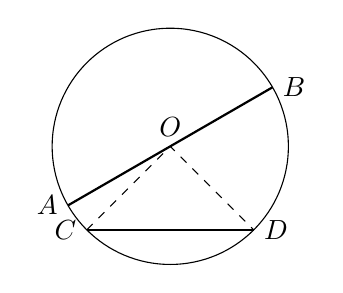
\begin{tikzpicture}
        \draw (0,0) circle (1.5);
\draw[thick] (-150:1.5)node[left]{$A$}--node[above]{$O$}(30:1.5)node[right]{$B$};
\draw[thick]  (-135:1.5)node[left]{$C$}--(-45:1.5)node[right]{$D$};
\draw[dashed](-135:1.5)--(0,0)--(-45:1.5);
    \end{tikzpicture}
\end{center}
\end{enumerate}
\end{ex}

\subsection{不共线的三点确定一圆}
我们已知,如果知道了圆心的位置和半径长,那么圆的
位置和大小也就确定了。现在我们来研究经过一个点;经过
两个点;经过三个点可分别作出几个圆?
    
已知一个点$A$, 很明显,以$A$点以外的任何点为圆心,
以这点到$A$点的距离为半径所作的圆都经过$A$点(图4.5)。
因此,\textbf{经过一点可以作无数个圆}。
\begin{figure}[htp]\centering
	\begin{minipage}[t]{0.48\textwidth}
		\centering
		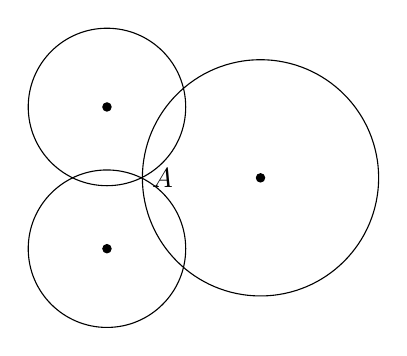
\begin{tikzpicture}[>=latex, scale=1]
\draw (0,.9) circle (1);
\draw (0,-.9) circle (1);
\draw (1.95,0) circle (1.5);
\foreach \x/\y in{0/.9, 0/-.9, 1.95/0}
{
    \draw (\x,\y)[fill=black]circle(1.5pt);
}
\node at (1.95-1.5,0)[right]{$A$};

		\end{tikzpicture}
		\caption{}
	\end{minipage}
	\begin{minipage}[t]{0.48\textwidth}
		\centering
		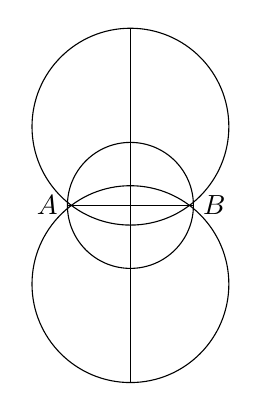
\begin{tikzpicture}[>=latex, scale=1]
	\draw (0,1) circle (1.25);
	\draw (0,-1) circle (1.25);
	\draw (0,0) circle (.8);	
	\draw (-.8,0)node[left]{$A$}--(.8,0)node[right]{$B$}   ;	
	\draw(0,2.25)--(0,-2.25);
		\end{tikzpicture}
		\caption{}
	\end{minipage}
\end{figure}

经过两个已知点$A$、$B$,可以作多少个圆呢(图4.6)?
由于经过$A$、$B$两点的圆的圆心到$A$点与$B$点的距离应相等,而
和$A$、$B$两点距离相等的点仅在$AB$的垂直平分线上,所以,
以$AB$的垂直平分线上任一点为圆心,以这点到$A$点(或$B$
点)的距离为半径所作的圆都经过$A$、$B$两点。因此,\textbf{经过
两点也可以作无数个圆,且圆心都在连结这两点的线段的垂
直平分线上}。

现在我们来研究,经过$A$、$B$、$C$三点可以作多少个圆的
问题?

\begin{figure}[htp]\centering
	\begin{minipage}[t]{0.48\textwidth}
		\centering
		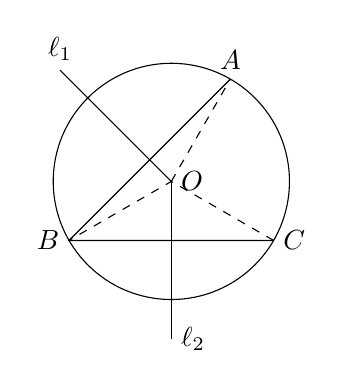
\begin{tikzpicture}[>=latex, scale=1]
\draw (0,0)node[right]{$O$} circle (1.5);
\draw[dashed] (-30:1.5)node[right]{$C$}--(0,0)--(-150:1.5)node[left]{$B$};
\draw (-30:1.5)--(-150:1.5)--(60:1.5);
\draw[dashed] (0,0)--(60:1.5)node[above]{$A$};
\draw (0,0)--(-90:2)node[right]{$\ell_2$};
\draw (0,0)--(135:2)node[above]{$\ell_1$};
		\end{tikzpicture}
		\caption{}
	\end{minipage}
	\begin{minipage}[t]{0.48\textwidth}
		\centering
		\begin{tikzpicture}[>=latex, scale=1]
\draw (0,0)--(5,0);
\foreach \x/\xtext in{1/A,2.5/B,4.5/C}
{
    \draw (\x,0)node[below]{$\xtext$}[fill=black] circle(1.5pt) ;
}
\draw[thick] (1.5,-1.5)--(1.5,1.5)node[above]{$\ell_1$};
\draw[thick] (4,-1.5)--(4,1.5)node[above]{$\ell_2$};
		\end{tikzpicture}
		\caption{}
	\end{minipage}
\end{figure}

我们知道,经过$A$、$B$两点的圆的圆心必定在$\overline{AB}$的垂
直平分线上(图4.7中的$\ell_1$),经过$B$、$C$两点的圆的圆心
又必定在$\overline{BC}$的垂直平分线上(图4.7中的$\ell_2$),因而经过
$A$、$B$、$C$三点的圆的圆心必定是直线$\ell_1$和$\ell_2$的交点$O$, 由
于$\overline{OA}=\overline{OB}=\overline{OC}$, 所以以$O$为圆心$\overline{OA}$为半径的圆经过
$A$、$B$、$C$三点。

这样一来,能不能说经过三个点就可作一个圆呢?我们
再来看图4.8中所示的三点$A$、$B$、$C$,它们是在同一条直线
上的,这时$\overline{AB}$和$\overline{BC}$的垂直平分线$\ell_1$和$\ell_2$都垂直于同一条直
线,于是$\ell_1\parallel \ell_2$, $\ell_1$和$\ell_2$便没有交点,这就说明了经过$A$、
$B$、$C$三点的圆的圆心根本不存在,所以也就没有圆都经过
$A$、$B$、$C$三点。因此,我们不能笼统地说经过三个点可作一
个圆。如果$A$、$B$、$C$三点在同一条直线上(叫做共线的点),
便没有圆经过这三点;如果$A$、$B$、$C$三点不在同一条直线
上(叫做不共线的点),那么$\overline{AB}$与
$\overline{BC}$的垂直平分线必相交
(为什么?),这时,就可作一个圆经过这三点,又由于
$\overline{AB}$和$\overline{BC}$的垂直平分线都只有一条,所以它们的交点也是唯
一的,从而$\overline{OA}$的长也是唯一的,所以经过$A$、$B$、$C$三点也
只能作一个圆。

于是,我们便得到确切的结论:

\begin{blk}{定理}
过不共线的三个点,可以作一个圆且只可以作一
个圆。    
\end{blk}
 
由上述讨论,我们还可看到一个圆的圆心到圆的任一条
弦的两个端点的距离相等,因而可得:

\begin{blk}{推论1}
圆的任一条弦的垂直平分线都通过圆心。
\end{blk}
 
由于任一个$\triangle ABC$的三个顶点不共线,因此经过$A$、$B$、
$C$三个顶点可以作一个圆,且只可以作一个圆$\odot O$(图4.9),这个圆叫做$\triangle ABC$的\textbf{外接圆},它的圆心$O$叫做$\triangle ABC$的\textbf{外心},而$\triangle ABC$叫做$O$的\textbf{内接三角形}。由于$\overline{OA}=\overline{OB}=\overline{OC}$, 
$O$点一定在三边的垂直平分线上,于是又可得:

\begin{figure}[htp]
    \centering
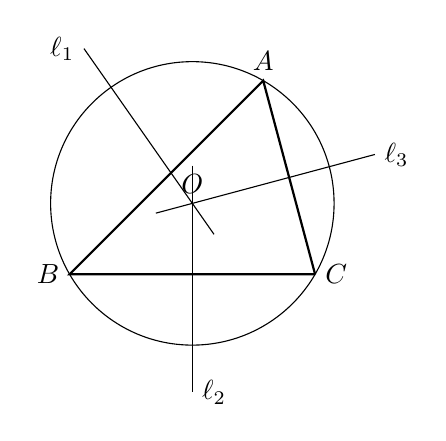
\begin{tikzpicture}[>=latex, scale=1.2]
\draw (0,0)node[above]{$O$} circle (1.5);
\draw[thick] (-30:1.5)node[right]{$C$}--(-150:1.5)node[left]{$B$}--(60:1.5)node[above]{$A$}--(-30:1.5);
\draw(0,.4)--(0,-2)node[right]{$\ell_2$};
\draw(15+180:.4)--(15:2)node[right]{$\ell_3$};
\draw(125-180:.4)--(125:2)node[left]{$\ell_1$};

    \end{tikzpicture}
    \caption{}
\end{figure}

\begin{blk}{推论2}
    三角形的三边的垂直平分线相交于一点,这个
点就是三角形的外心。
\end{blk}
 
由推论2我们又可得到:
 
\begin{blk}{推论3}
   三角形的三条高线相交于一点。
\end{blk}

已知:$AD$、$BE$、$CF$是$\triangle ABC$的三条高线(图4.10)。
求证:$AD$、$BE$、$CF$相交于一点。

\begin{figure}[htp]
    \centering
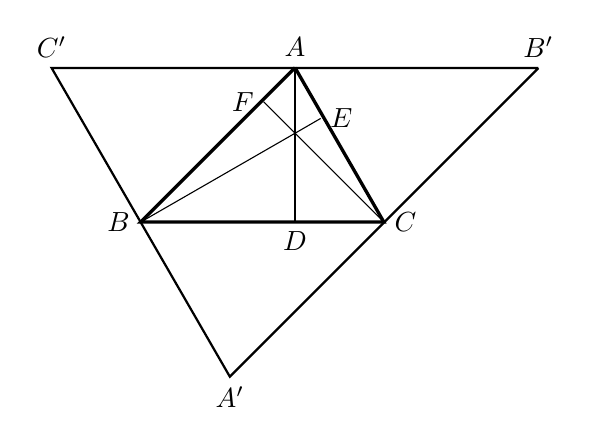
\begin{tikzpicture}[scale=.8]
\draw[thick] (15:4)node[above]{$B'$}--(180-15:4)node[above]{$C'$}--(-90-15:4)node[below]{$A'$}--(15:4);
\draw[very thick] (0,1.04)node[above]{$A$}--(-2.45,-1.41)node[left]{$B$}--(1.41,-1.41)node[right]{$C$}--(0,1.04);
\draw (0,1.04)--(0,-1.41)node[below]{$D$};
\draw (-2.45,-1.41)--(0,0)--(0.406,.235)node[right]{$E$};
\draw (1.41,-1.41)--(0,0)--(-.5,.5)node[left]{$F$};
\end{tikzpicture}
    \caption{}
\end{figure}

\begin{proof}
    经过$\triangle ABC$的各顶点$A$、$B$、$C$分别作对边的平
行线,设它们分别相交于$B'$、$C'$、$A'$各点,于是$AD\bot B'C'$,
$BE\bot C'A'$, $CF\bot A'B'$(为什么?),又因为四边形$BCAC'$和
$BCB'A$都是平行四边形(为什么?)。

$\therefore\quad \overline{CA}=\overline{BC}=\overline{AB'}$, 于是$A$是$\overline{B'C'}$的中点。

同理,$B$是$\overline{A'C'}$的中点,$C$是$\overline{A'B'}$的中点,因此,$AD$、
$BE$、$CF$分别是$\triangle A'B'C'$的三边上的垂直平分线,由推论2
可知$AD$、$BE$和$CF$相交于一点。
\end{proof}


图4.10中,画出的是锐角三角形,如$\triangle ABC$是钝角三
角形,上述证明过程同样适用,同学可自己验证。

三角形的三条高线的交点叫做\textbf{三角形的垂心}。

\begin{example}
    求作一条已知弧的圆心。
\end{example}

已知$\wideparen{EF}$(图4.11).

求作:$\wideparen{EF}$所在圆的圆心。

作法
\begin{enumerate}
    \item 在$\wideparen{EF}$
    上任取三点$A$、$B$、$C$, 并且作$\overline{AB}$、$\overline{BC}$.
    \item 分别作$\overline{AB}$、$\overline{BC}$的垂直平分线$\ell_1$和$\ell_2$, 设它们
    的交点为$O$, $O$点就是所求作的圆心。
\end{enumerate}

\begin{proof}
    $\because\quad A$、$B$、$C$三点在$\wideparen{EF}$上(作法)

$\therefore\quad \wideparen{EF}$是经过$A$、$B$、$C$的圆的一部分。

又$\because\quad O$是经过$A$、$B$、$C$的圆的圆心,

$\therefore\quad O$是$\wideparen{EF}$所在圆的圆心。
\end{proof}

\begin{figure}[htp]\centering
    \begin{minipage}[t]{0.48\textwidth}
    \centering
  \begin{tikzpicture}[>=latex, scale=1]
\tkzDefPoint(150:2.5){A}
\tkzDefPoint(110:2.5){B}
\tkzDefPoint(40:2.5){C}
\tkzDefPoint(160:2.5){E}
\tkzDefPoint(20:2.5){F}
\tkzDrawSegments[very thick](A,B B,C)
\tkzDefPoints{0/0/O}
\tkzDefPointBy[projection = onto A--B](O)\tkzGetPoint{O'}
\tkzDefPointBy[projection = onto C--B](O)\tkzGetPoint{O''}
\tkzDrawLines[add=.3 and .7](O,O' O,O'')
\tkzAutoLabelPoints[center=O](A,B,C,E,F)
\tkzDrawArc[color=black, thick](O,F)(E)
\tkzLabelPoints[right](O)
\node at (-2,3){$\ell_1$};
\node at (1,3){$\ell_2$};
    \end{tikzpicture}
    \caption{}
    \end{minipage}
    \begin{minipage}[t]{0.48\textwidth}
    \centering
    \begin{tikzpicture}[>=latex, scale=1]
\tkzDefPoints{0/0/B, 4/0/C, 3/3/A}
\tkzDrawPolygon(A,B,C)
\tkzDefTriangleCenter[circum](A,B,C)  \tkzGetPoint{O}
\tkzDefTriangleCenter[ortho](A,B,C)  \tkzGetPoint{H}
\tkzDefPointBy[projection= onto B--C](O) \tkzGetPoint{L}
\tkzDefPointBy[projection= onto B--A](O) \tkzGetPoint{M}
\tkzInterLL(A,C)(B,H)\tkzGetPoint{B'}
\tkzInterLL(B,C)(A,H)\tkzGetPoint{D}
\tkzInterLL(A,B)(C,H)\tkzGetPoint{C'}
\tkzDefMidPoint(B,H) \tkzGetPoint{K}
\tkzDrawSegments(A,D C,C' B,B' O,M O,L M,K L,K)
\tkzLabelPoints[below](B,C,L,D)
\tkzLabelPoints[above](A,M)
\tkzLabelPoints[right](O)
\tkzLabelPoints[above right](H)
\tkzLabelPoints[above left](K)
\tkzDrawPoints(O,H,K)
    \end{tikzpicture}
    \caption{}
    \end{minipage}
    \end{figure}

\begin{example}
    已知$O$和$H$各是$\triangle ABC$的外心和垂心,$OL\bot \overline{BC}$
    于$L$(图4.12). 
    求证:$\overline{OL}=\frac{1}{2}\overline{AH}$
\end{example}

\begin{proof}
    已知$OL\bot \overline{BC}$于$L$点,作$OM\bot \overline{AB}$于$M$点,由
    于$O$是$\triangle ABC$的外心,所以$L$、$M$分别是$\overline{BC}$、$\overline{AB}$的中点。
    取$\overline{BH}$的中点$K$, 作$\overline{MK}$, $\overline{LK}$, 
 
$\because\quad     MK\parallel AH,\quad OL\parallel AH$,

$\therefore\quad MK\parallel OL$,

同理可证,$LK\parallel OM$,

$\therefore\quad OMKL$是平行四边形,

$\therefore\quad \overline{OL}=\overline{MK}=\frac{1}{2}\overline{AH}$
\end{proof}

\begin{ex}
\begin{enumerate}
    \item 分别作一个锐角三角形、一个直角三角形和一个钝角三
    角形的外接圆,并说出它们的外心的位置各有什么特点。
    \item 经过任意四点,可不可以作一个圆?试举例说明。
    \item 分别作出一个锐角三角形、一个直角三角形和一个钝角
    角形的套心,并说出它们的位置各有什么特点。
    \item 已知$H$是$\triangle ABC$的垂心,
    $D$、$E$、$F$是三高的垂足。试分别说出$\triangle HBC$、$\triangle HAC$、$\triangle HAB$的垂心各是图中哪一点。
\end{enumerate}
\end{ex}

\begin{figure}[htp]
    \centering
\begin{tikzpicture}
    \tkzDefPoints{0/0/B, 4/0/C, 1.8/2.5/A}
\tkzDrawPolygon(A,B,C)
\tkzDefTriangleCenter[ortho](A,B,C)  \tkzGetPoint{H}
\tkzInterLL(A,C)(B,H)\tkzGetPoint{E}
\tkzInterLL(B,C)(A,H)\tkzGetPoint{D}
\tkzInterLL(A,B)(C,H)\tkzGetPoint{F}
\tkzDrawSegments(A,D B,E C,F)
\tkzLabelPoints[below](B,C,D)
\tkzLabelPoints[left](F)
\tkzLabelPoints[right](E)
\tkzLabelPoints[above](A)
\tkzLabelPoints[below right](H)
\end{tikzpicture}
    \caption*{第4题}
\end{figure}

\subsection{圆的对称性}
已知$\odot O$(图4.13), 在$O$上任取一点$A$, 引直径$\overline{AA'}$, 
则$\overline{AA'}$被圆心$O$平分.这就是说$A'$是以点$O$为对称中心的
点$A$的对称点,如果在$\odot O$上再取$B,C,D,\ldots$, 并引直径
$\overline{BB'},\overline{CC'},\overline{DD'},\ldots$, 那么点$B',C',D',\ldots$ 也都分别是
以$O$为对称中心的点$B,C,D,\ldots$的对称点。这就说明
了$\odot O$上以$O$为对称中心的任何点的对称点都在$\odot O$上。由
此可知:\textbf{圆是中心对称形;圆心是它的对称中心}。

已知$\overline{AA'}$是$\odot O$的任一条直径(图4.14),作直径$\overline{BB'}\bot 
\overline{AA'}$, 把$\odot O$左边部分沿着直线$AA'$翻折过来,由于$\overline{BB'}\bot \overline{AA'}$, $\overline{OB'}=\overline{OB}$, 那么$B$点就与$B'$点重合,因为经过$A$、
$B'$、$A'$三点只可以作一个圆,所以以$A$、$A'$为端点,经过
$B'$点的弧只有一条,因此$\wideparen{ABA'}$与
$\wideparen{AB'A'}$重合。由此可知,
圆是轴对称图形,任一条通过圆心的直线都是它的对称轴。

\begin{figure}[htp]\centering
    \begin{minipage}[t]{0.48\textwidth}
    \centering
  \begin{tikzpicture}[>=latex, scale=1]
\tkzDefPoint(20:1.5){A'}
\tkzDefPoint(-30:1.5){B'}
\tkzDefPoint(200:1.5){A}
\tkzDefPoint(150:1.5){B}
\tkzDefPoint(90:1.5){C}
\tkzDefPoint(-90:1.5){C'}
\tkzDefPoint(0,0){O}
\tkzDrawCircle[very thick](O,A)
\tkzDrawSegments[thick](A,A' B,B' C,C')
\tkzAutoLabelPoints[center=O](A,A',B,B',C,C')
\tkzLabelPoints[above right](O)
    \end{tikzpicture}
    \caption{}
    \end{minipage}
    \begin{minipage}[t]{0.48\textwidth}
    \centering
    \begin{tikzpicture}[>=latex, scale=1]
      \tkzDefPoint(0:1.5){B'}
\tkzDefPoint(180:1.5){B}
\tkzDefPoint(90:1.5){A}
\tkzDefPoint(-90:1.5){A'}
\tkzDefPoint(0,0){O}
\tkzDrawCircle[very thick](O,A)
\tkzDrawSegments[thick](A,A' B,B')
\tkzAutoLabelPoints[center=O](B,B')
\draw[dashed](A)node[above right]{$A$}--(0,2.5);
\draw[dashed](A')node[below right]{$A'$}--(0,-2.5);
    \end{tikzpicture}
    \caption{}
    \end{minipage}
    \end{figure}

由上述圆的对称性,我们可推出许多圆的重要性质。

\begin{blk}
    {推论1} 圆被它的任何一条直径截出的两段弧相等。这两
段弧都叫做半圆。
\end{blk}

小于半圆的弧叫做\textbf{劣弧},大于半圆的弧叫做\textbf{优弧}。以后
说到弧,如不特别指明,一般都指的是劣弧。

\begin{blk}
    {推论2} 一圆的直径垂直于一条非直径的弦的充分必要
条件是这直径平分这条弦或平分这条弦所对的弧。
\end{blk}

我们来证必要性,充分性留给同学们自证。

已知:$\odot O$中,直径$\overline{CD}\bot $弦$\overline{AB}$于$E$点(图4.15).

求证:$\overline{AE}=\overline{BE}$, $\wideparen{AD}=\wideparen{BD}$, $\wideparen{AC}=\wideparen{BC}$.

\begin{proof}
$\because\quad \overline{CD}$是$\odot O$的直径

$\therefore\quad $直线$CD$是$\odot O$的对称轴。

又$\because\quad CD\bot AB$于$E$点

$\therefore\quad CD$也是等腰$\triangle OAB$的
对称轴。以$CD$为轴把图形翻
折叠合时,半圆$\wideparen{CAD}$与半圆$\wideparen{CBD}$重合,$\overline{AE}$与
$\overline{BE}$
重合。$A$点与$B$点重合,
$\wideparen{AD}$与$\wideparen{BD}$, $\wideparen{AC}$与
$\wideparen{BC}$都重合

$\therefore\quad \overline{AE}=\overline{BE},\quad 
\wideparen{AD}=\wideparen{BD},\quad 
\wideparen{AC}=\wideparen{BC}$.
\end{proof}

\begin{figure}[htp]\centering
    \begin{minipage}[t]{0.48\textwidth}
    \centering
  \begin{tikzpicture}[>=latex, scale=1]
\tkzDefPoints{0/0/O, 0/2/C, 0/-2/D}
\tkzDefPoint(-30:2){B}
\tkzDefPoint(-150:2){A}
\tkzAutoLabelPoints[center=O](A,B,C,D)
\tkzLabelPoints[above left](O)
\tkzInterLL(O,D)(A,B)\tkzGetPoint{E}
\tkzLabelPoints[above right](E)
\tkzDrawSegments(A,B C,D A,O B,O)
\tkzDrawCircle[thick](O,C)
    \end{tikzpicture}
    \caption{}
    \end{minipage}
    \begin{minipage}[t]{0.48\textwidth}
    \centering
    \begin{tikzpicture}[>=latex, scale=1]
\tkzDefPoints{0/0/O, 0/3.5/C, 0/-1/D, 0/2/E}
\tkzDefPoint(30:2){B}
\tkzDefPoint(150:2){A}
\tkzDrawLines[add=.1 and .1](C,D)
\tkzLabelPoints[right](C,D)
\tkzLabelPoints[below](A,B)
\tkzLabelPoints[below right](E)
\tkzDrawArc[thick, color=black](O,B)(A)
\tkzDrawSegments[thick](A,B)
\tkzCompasss(A,C B,C A,D B,D)


    \end{tikzpicture}
    \caption{}
    \end{minipage}
    \end{figure}



\begin{example}
    平分一条已知弧。

已知:$\wideparen{AB}$(图4.16).

求作:平分$\wideparen{AB}$的点。

作法
\begin{enumerate}
    \item 作$\overline{AB}$
    \item 作$\overline{AB}$的垂直平分线$CD$交$\wideparen{AB}$于$E$点。则$E$点就
是所求作的点。
\end{enumerate}
\end{example}

\begin{proof}
$\because\quad CD$是$\overline{AB}$的垂直平分线(作法)。

$\therefore\quad CD$ 必通过圆心,

$\therefore\quad \wideparen{AE}=\wideparen{BE}$ (推论2).

$\therefore\quad E$点平分$\wideparen{AB}$.
\end{proof}

\begin{example}
    已知大小两圆有公共圆心$O$, 大圆的弦交小圆于
$C$、$D$ (图4.17).

求证:$\overline{AC}=\overline{BD}$.
\end{example}

\begin{proof}
    作$\overline{OM}\bot \overline{AB}$于$M$点,则$\overline{AM}=\overline{BM}$, $\overline{CM}=\overline{DM}$.

$\therefore\quad     \overline{AM}-\overline{CM}=\overline{BM}-\overline{DM}$.
    
$\therefore\quad \overline{AC}=\overline{BD}$
\end{proof}

\begin{figure}[htp]\centering
    \begin{minipage}[t]{0.48\textwidth}
    \centering
  \begin{tikzpicture}[>=latex, scale=1]
\tkzDefPoints{0/0/O, 0/-1/M, -1.5/-1/A, 1.5/-1/B, -1/-1/C, 1/-1/D}
\tkzDrawCircle[thick](O,C)
\tkzDrawCircle[thick](O,A)
\tkzDrawSegments[thick](A,B O,M)
\tkzLabelPoints[below](A,B,C,D,M)
\tkzLabelPoints[above](O)

    \end{tikzpicture}
    \caption{}
    \end{minipage}
    \begin{minipage}[t]{0.48\textwidth}
    \centering
    \begin{tikzpicture}[>=latex, scale=1]
\tkzDefPoints{0/0/O}
\tkzDefPoint(45:1.8){B}
\tkzDefPoint(135:1.8){A}
\tkzDefPoint(-30:1.8){D}
\tkzDefPoint(-150:1.8){C}
\tkzDefMidPoint(A,B)\tkzGetPoint{E}
\tkzDefMidPoint(C,D)\tkzGetPoint{F}
\tkzAutoLabelPoints[center=O](A,B,C,D)
\tkzLabelPoints[above](E)
\tkzLabelPoints[below](F)
\tkzDrawSegments(A,O C,O A,B C,D E,F)
\tkzLabelPoints[right](O)
\tkzDrawCircle[thick](O,A)
    \end{tikzpicture}
    \caption{}
    \end{minipage}
    \end{figure}

    
\begin{example}
    已知$\odot O$的两条平行弦$\overline{AB}=6$cm, $\overline{CD}=8$cm
    且
    $AB$和$CD$间的距离是7cm, 求$\odot O$的半径长(图4.18).
\end{example}

\begin{solution}
    作$OE\bot \overline{AB}$
于$E$点,延长$\overline{EO}$交$\overline{CD}$于$F$点。

$\because\quad AB\parallel CD$,

$\therefore\quad OF\bot CD$,

$\therefore\quad \overline{EF}$为$\overline{AB}$和$\overline{CD}$的公垂线段,且$\overline{EF}=7$cm,
$\overline{AE}=\frac{1}{2}\overline{AB}=3$cm, $\overline{CF}=
\frac{1}{2}\overline{CD}=4$cm.

设$\overline{OA}=\overline{OC}=x$, $\overline{OE}=y$, 则由勾股定理可得方程组:
\[\begin{cases}
    x^2=3^2+y^2\\
    x^2=(7-y)^2+4^2
\end{cases}\]
解这个方程组,舍去不合理的根得:
\[\begin{cases}
    x=5\\y=4
\end{cases}\]

答:$\odot O$的半径是5cm.
\end{solution}

\begin{ex}
\begin{enumerate}
    \item 把本节推论2用“若一则”
    形式写出互逆的定理。
    \item 作出图中圆的圆心。
    \item 已知$\odot(0,5{\rm cm})$, 它的一条弦$\overline{AB}=8$cm, 点$M$是
    $\overline{AB}$的
    中点,求$\overline{OM}$的长。
    \item 已知一圆的半径是25cm, 一弧所对的弦长是48cm, 求这
    弧的一半所对的弦长。
    \item 求证圆中的非直径的两弦必不能互相平分
    (提示:用反证法)。
\end{enumerate}
\end{ex}

\begin{figure}[htp]
    \centering
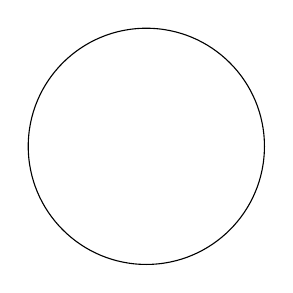
\begin{tikzpicture}
    \draw(0,0) circle (1.5);
\end{tikzpicture}
    \caption*{第2题}
\end{figure}

\subsection{弧、弦和弦心距之间的关系}
圆的圆心到一条弦的距离,叫做这条弦的弦心距,例如
在图4.19中,$\overline{AB}$是$\odot O$的一条弦,$\overline{OE}\bot \overline{AB}$于$E$点,$\overline{OE}$
的长就是弦
$\overline{AB}$的弦心距。下面我们来学习弧、弦和弦心距
之间的关系。

\begin{blk}
    {定理} 在同圆或等圆中,两条弧相等的充要条件是它们
所对的弦相等,或它们所对的弦的弦心距相等。
\end{blk}

\begin{figure}[htp]
    \centering
    \begin{tikzpicture}[>=latex]
 \tkzDefPoints{0/0/O}
\tkzDefPoint(-60:2){B}
\tkzDefPoint(-120:2){A}
\tkzDefPoint(0:2){C}
\tkzDefPoint(60:2){D}
\tkzDefMidPoint(A,B)\tkzGetPoint{E}
\tkzDefMidPoint(C,D)\tkzGetPoint{F}
\tkzDrawSegments[very thick](A,B C,D)
\tkzDrawSegments(O,A O,B O,C O,D O,E O,F)
\tkzLabelPoints[above left](O)
\tkzAutoLabelPoints[center=O](A,B,C,D)
\tkzLabelPoints[above right](E)
\tkzLabelPoints[left](F)
\tkzDrawCircle[thick](O,A)       

\draw[->](-50:1.2) arc (-50:-10:1.2);
    \end{tikzpicture}
    \caption{}
\end{figure}

我们来证条件的必要性,充分性由同学们自证:

已知:在$\odot O$中,$\wideparen{AB}=\wideparen{CD}$, 
$OE\bot  AB$于$E$点,$OF\bot CD$于
$F$点(图4.19)。

求证:$\overline{AB}=\overline{CD}$, $\overline{OE}=\overline{OF}$.

\begin{proof}
    作半径$\overline{OA}$、$\overline{OB}$、$\overline{OC}$、$\overline{OD}$. 把$\wideparen{AB}$连同经过
两端的半径绕着$O$点,依箭头所指的方向旋转,使半径$\overline{OA}$
和半径$\overline{OC}$重合。

$\because\quad \wideparen{AB}=\wideparen{CD}$.

$\therefore\quad \wideparen{AB}$与$\wideparen{CD}$重合,弦$\overline{AB}$与弦$\overline{CD}$重合。

又$\because\quad $从一点到一条直线只可以作一条垂线,

$\therefore\quad \overline{OE}$与$\overline{OF}$
也重合

$\therefore\quad \overline{AB}=\overline{CD},\quad \overline{OE}=\overline{OF}$.
\end{proof}

对于等圆情况的证明,只要使两圆重合就可以了。

这个定理告诉我们,在同圆或等圆中,“弧相等”、
“弦相等”、“弦心距相等”它们当中只要有一个是对的,
其它两个也一定是对的。这就是说:

\begin{blk}
   “弧相等”$\Longleftrightarrow$“弦相等”$\Longleftrightarrow$“弦心距相等” 
\end{blk}

\begin{example}
    已知(图4.20),$\overline{OE}$是$\odot O$中的半径,$F$是$\overline{OE}$上任一
点,$\overline{AB}$和$\overline{CD}$为过$F$点的弦且$\angle AFO=\angle DFO$.

求证:$\overline{AB}=\overline{CD}$
\end{example}

\begin{proof}
作$\overline{OM}\bot \overline{AB}$于$M$点,$\overline{ON}\bot \overline{CD}$ 于$N$点,在直角
$\triangle OMF$与直角$\triangle ONF$中,

$\because\quad \angle MFO=\angle NFO,\quad \overline{OF}=\overline{OF}$.

$\therefore\quad \triangle OMF\cong \triangle ONF$

$\therefore\quad \overline{OM}=\overline{ON}$.

$\therefore\quad \overline{AB}=\overline{CD}$.
\end{proof}





\begin{example}
    
\end{example}

\begin{solution}
    
\end{solution}

\begin{example}
    
\end{example}


\begin{solution}
    
\end{solution}

\begin{example}
    
\end{example}


\begin{solution}
    
\end{solution}


\begin{example}
    
\end{example}

\begin{solution}
    
\end{solution}



\begin{example}
    
\end{example}

\begin{solution}
    
\end{solution}
\begin{example}
    
\end{example}

\begin{solution}
    
\end{solution}

\begin{example}
    
\end{example}

\begin{solution}
    
\end{solution}































































































































































































\begin{example}
    已知扇形的半径$r\approx 4.8$cm, 所含的圆心角是
$42^{\circ}$, 求它的周长和面积($\pi \approx 3.14$).
\end{example}

\begin{solution}
    设扇形的弧长为$\ell$, 则:
    \[\ell=\frac{42\x3.14\x4.8}{180}\approx 3.5({\rm cm})\]
$\therefore\quad $扇形的周长$=2r+\ell=2\x4.8+3.5=13.1$(cm).

扇形的面积$=\frac{1}{2}\ell r=\frac{1}{2}\x3.5\x4.8\approx 8.4({\rm cm^2})$

答:扇形周长约是13.1cm, 面积约为8.4${\rm cm^2}$.
\end{solution}

\begin{ex}
\begin{enumerate}
\item 已知圆的周长$C\approx 48.5$cm, 求圆的半径$r$.
\item 一列火车,火车头上的主动轮的直径约是1.2米,如果主
动轮每秒钟转250次,那么,火车的速度是每小时约多少
公里?
\item 圆的半径约是8.2cm, 圆心角是$32^{\circ}30'$, 求圆心角所对
的弧长。
\item 已知扇形的半径是4.2cm, 所含的弧是$35^{\circ}$, 求它的周长
和面积。
\end{enumerate}
\end{ex}

\subsection*{习题4.4}
\begin{enumerate}
    \item 求作已知圆的外切正六边形。

    \item 已知一边,求作正八边形。
    \item 我国民间相传有正五边形的近似画法:“九五顶五九,八、五两边分”它的意义如图所示
\begin{enumerate}
    \item 按照图中注明的尺寸,计算这五边形各边的长。
    \item 用这种方法作边长是30mm的正五边形。
\end{enumerate}

\begin{figure}[htp]
    \centering
    \begin{tikzpicture}[scale=.25, >=latex]
\tkzDefPoints{-8/0/A, 8/0/B, -5/-9.5/C, 5/-9.5/D, 0/5.9/E}
\tkzDrawPolygon(E,A,C,D,B)
\draw[<->](A)--node[fill=white]{8寸}(0,0);
\draw[<->](B)--node[fill=white]{8寸}(0,0);
\draw(C)--node[above]{5寸}(0,-9.5);
\draw(D)--node[above]{5寸}(0,-9.5);
\draw[<->](E)--node[fill=white]{5.9寸}(0,0);
\draw[<->](0,-9.5)--node[fill=white]{9.5寸}(0,0);
    \end{tikzpicture}
    \caption{}
\end{figure}

\item 用全等的正多边形的砖铺地面,要砖与砖之间不留空隙,有哪几种正多边形的砖合用?
\item 已知圆的半径为$r$. 求外切正三角形、外切正方形、外
切正六边形的周长和面积。
\item 求证:正三角形的边心距、半径和高的比是$1:2:3$.
\item 已知圆的半径是$r$, 求证圆的内接正八多边形的周长是
$8\sqrt{2-\sqrt{2}}r$, 面积是$2\sqrt{2}r^2$.
\item 已知正三角形外接圆面积是100平方厘米,求它的内切
圆面积。
\item 有一圆管的外直径是150mm, 内直径是100mm, 求这圆
管的横断面的面积和它的厚度。
\item 已知一圆的半径是200mm, $AB$所对的圆心角是$45^{\circ}$, 求
$\wideparen{AB}$长和扇形$OAB$的面积。
\item 如图:$\triangle ABC$中,$\angle C=90^{\circ}$, $\wideparen{ACB}$是以$\overline{AB}$为直径的半
圆,$\wideparen{ADC}$是以$\overline{AC}$为直径的半圆,$\wideparen{CEB}$是以$\overline{CB}$为直径
的半圆。

求证:I的面积$+$II的面积$=$III的面积。

\begin{figure}[htp]\centering
    \begin{minipage}[t]{0.48\textwidth}
    \centering
\begin{tikzpicture}[>=latex, scale=.9]
    \tkzDefPoints{0/0/A, 5/0/B, 3.2/2.4/C}
    \tkzDrawSemiCircle[pattern=north west lines,diameter](A,C)
\tkzDrawSemiCircle[pattern=north west lines,diameter](C,B)
\tkzDrawSemiCircle[fill=white,diameter](A,B)
\tkzDrawPolygon[pattern=north east lines](A,B,C)
\tkzLabelPoints[below](A,B)
\tkzLabelPoints[above](C)
\node at (3,1)[fill=white]{III};
\node at (1,2.6)[fill=white]{I};
\node at (5,1.5)[fill=white]{II};


    \end{tikzpicture}
    \caption{}
    \end{minipage}
    \begin{minipage}[t]{0.48\textwidth}
    \centering
    \begin{tikzpicture}[>=latex, scale=1.3]
\tkzDefPoints{0/0/A, 1.732/0/B, 0/-1.5/O_1, 1.732/-.5/O_2}
\tkzDrawCircle[thick](O_1,A)  \tkzDrawCircle[thick](O_2,B)
\draw(A)--node[left]{3}(O_1);
\draw(B)--node[left]{1}(O_2);
\tkzDefPointsBy[reflection = over O_1--O_2](A,B){A',B'}
\tkzDrawSegments(A,B A',B')

    \end{tikzpicture}
    \caption{}
    \end{minipage}
    \end{figure}


\item 为了把半径是3cm和1cm的两根圆柱紧紧地捆扎在一
起,绕一圈需要多少铅丝?
\end{enumerate}

\section*{复习题四}
\begin{enumerate}
    \item 已知两定点$A$、$B$, 分别以$A$、$B$为圆心,以同一的半
径$r\; \left(r\ge \frac{1}{2}\overline{AB}\right)$
作圆,求证这些等圆的交点都在$\overline{AB}$
的垂直平分线上。
\item 两圆的半径都是4cm, 并且一圆过另一圆的圆心,求这
两圆的公共弦长。
\item 已知$\overline{AB}$是$O$的直径,以$\overline{OB}$为直径作$O'$, 过$B$点
作直线与$O$相交于$M$点,与$CO'$相交于$N$点。
求证:$\overline{BN}=\overline{MN}$.
\item 已知$\overline{CD}$是$\odot O$的直径,$A$为$\odot O$外一点,$AT$切圆于$T$
点,如果切点$T$与$C$的连线平行于$AO$, 求证$AD$与$\odot O$相切。
\item 以$O$为圆心作两个同心圆,已知$\overline{AB}$为小圆的直径,过
$A$、$B$两点分别作小圆的切线交大圆于$C$、$D$两点:(使
$C$、$D$分别在$\overline{AB}$的两侧),证明$C$、$O$、$D$三点共线。
\item 若一圆的两条切线交成$60^{\circ}$角,圆的半径为$r$, 求交点到
圆心的距离。若交角为$120^{\circ}$, 交点到圆心的距离又是多 
少?
\item 有一桥拱是圆弧$\wideparen{ACB}$, 桥的跨度$\overline{AB}=37.4$米,拱高
$\overline{CD}=7.2$米,求拱圈的半径。


\begin{figure}[htp]\centering
    \begin{minipage}[t]{0.48\textwidth}
    \centering
\begin{tikzpicture}[>=latex, scale=1]
\tkzDefPoints{-2.5/0.5/A_1, 2.5/0.5/B_1, -1.5/2.25/D_1, 1.5/2.25/C_1}
\tkzDrawPolygon[pattern=bricks](A_1,B_1,C_1,D_1)
\fill[white] (-1.75,0) arc (180:0:1.75);
\tkzDefPoints{0/1.75/C, 0/.5/D, 0/0/O}
\tkzInterLC(A_1,B_1)(O,C) \tkzGetPoints{A}{B}
\tkzDrawSegments[dashed](A,B C,D)
\tkzLabelPoints[below](A,B,D)
\tkzLabelPoints[below right](C)
\draw(C) arc (90:90-73.4:1.75);
\draw(C) arc (90:90+73.4:1.75);
    \end{tikzpicture}
    \caption*{第7题}
    \end{minipage}
    \begin{minipage}[t]{0.48\textwidth}
    \centering
    \begin{tikzpicture}[>=latex, scale=1.5]
\fill[pattern=north east lines](0,0) circle (1);
\fill[white](-.5,.25) rectangle (.5,1.2);
\draw(0,0) circle(1);
\draw(0,0)--node[below]{$r$}(170:1);
\foreach \x in {.25,0.866}
{
    \draw(0.5,\x)--(1.5,\x);
}
\draw(0,-1)--(1.5,-1);
\draw[<->](1.3,.25)--node[fill=white]{$x$}(1.3,.866);
\draw[<->](1.3,.25)--node[fill=white]{$b$}(1.3,-1);
\draw(-.5,1.25)--(-.5,.25)--(.5,.25)--(.5,1.25);
\draw[<->](-.5,1.15)--node[fill=white]{$a$}(.5,1.15);

    \end{tikzpicture}
    \caption*{第8题}
    \end{minipage}
    \end{figure}

\item 如图,一工件的断面,$a$、$b$、$r$为已知,求
$x$.
\item 已知$\overline{AB}$为一半圆的直径,直线$\ell$与半圆相切于$C$点,
$\overline{CD}\bot\overline{AB}$于$D$点,$\overline{AM}\bot \ell$于$M$点,$\overline{BN}\bot \ell$于$N$点。

求证:$\overline{MC}=\overline{NC}$;$\overline{CD}^2=\overline{AM}\cdot \overline{BN}$.

\item 已知$\odot O_1$与$\odot O_2$外切于$A$点,一直线与$\odot O_1$和$\odot O_2$分
别相切于$T_1$、$T_2$两点,并与连心线$O_1O_2$相交于$S$点,

求证:$\overline{SA}^2=\overline{ST_1}\cdot \overline{ST_2}$.
\item 已知$\overline{MN}$为一圆的直径,过圆外一点$D$作$\overline{DA}\bot \overline{MN}$于
$A$点交圆于$C$点,
$\overline{DN}$交圆于$P$, $\overline{MP}$交$\overline{AD}$于$B$, 求
证:$\overline{AC}^2=\overline{AB}\cdot \overline{AD}$(提示:先证$\overline{AB}\cdot \overline{AD}=\overline{AM}\cdot 
\overline{AN}$)。
\item 过两相交圆的公弦上的一点$P$, 作一条直线交一圆于
$A$、$B$两点与另一圆相交于$C$、$D$两点,
求证:$\overline{AC}:\overline{CP}=\overline{BD}:\overline{BP}$.
\item 设$\overline{AB}$是一圆的直径,由$A$、$B$两点作弦$\overline{AC}$及$\overline{BD}$
相交
于$E$点,求证:$\overline{AE}\cdot \overline{AC}+\overline{BE}\cdot \overline{BD}=\overline{AB}^2$.

(提示,过$E$作$EP\bot AB$于$P$, 寻找共圆点,利用圆幂
定理)
\item 在$\triangle ABC$中,$\angle A$的外角平分线与此三角形的外接圆
相交于$D$, 求证 $\overline{BD}=\overline{CD}$.
\item 假设两圆互相外切,求证以两圆心之间线段作直径的圆
必与前两圆的外公切线相切。
\item 知直角$\triangle ABC$, $\angle C=90^{\circ}$, 过$\overline{AC}$
边上一点$D$, 作斜
边$\overline{AB}$的垂线交斜边于$E$点,交它的外接圆于$G$点,交
$\overline{BC}$的延长线于$F$点,
求证:$\overline{EG}^2=\overline{EA}\cdot \overline{EB}$;$\overline{EG}^2=\overline{ED}\cdot \overline{EF}$.
\item 求证正三角形内的任一点到三边的距离和等于一边上的
高。
\item 求证:圆内接正$n$边形内任一点到各边的距离和等于$n$
倍边心距。
\item 已知等边$\triangle ABC$内接于$\odot O$, $P$为$\wideparen{BC}$上任一点. 
求证:$\overline{PA}=\overline{PB}+\overline{PC}$.
\item 从圆外一点$P$, 作这个圆的切线$PA$, $A$是切点,再从$P$
点引圆的割线与圆相交于$B$、$C$, 设$\angle P$的平分线与$\overline{AB}$、$\overline{AC}$
的交点分别是$D$、$E$. 

求证:$\frac{\overline{DB}}{\overline{AB}}+\frac{\overline{EC}}{\overline{AC}}=1$

\item 已知$\odot O$与$\odot O'$相离,连心线与$\odot O$和$\odot O'$的交点顺
次是$A$、$B$、$C$、$D$, 直线$PP'$分别与$\odot O$和$\odot O'$相切于
$P$、$P'$点,求证:$\overline{PP'}^2=\overline{AC}\cdot \overline{BD}$.
\end{enumerate}
